\documentclass[a4paper]{article}

\usepackage[english]{babel}
\usepackage[utf8]{inputenc}
\usepackage{amsmath}
\usepackage{graphicx}
\usepackage[colorinlistoftodos]{todonotes}

\usepackage{theorem}
\usepackage{amssymb}

\usepackage{hyperref}

\usepackage{caption}
\usepackage{subcaption}

\newenvironment{proof}{{\bf Proof:  }}{\hfill\rule{2mm}{2mm}}

\newtheorem{fact}{Fact}[section]
\newtheorem{lemma}[fact]{Lemma}
\newtheorem{theorem}[fact]{Theorem}
\newtheorem{definition}[fact]{Definition}
\newtheorem{corollary}[fact]{Corollary}
\newtheorem{proposition}[fact]{Proposition}
\newtheorem{claim}[fact]{Claim}
\newtheorem{exercise}[fact]{Exercise}

\newcommand{\RT}[1]{\marginpar{\footnotesize\color{red}RT: #1}}


\usepackage{tikz}
\usetikzlibrary{arrows}
\usepackage{amsmath}

% Defines a `datastore' shape for use in DFDs.  This inherits from a
% rectangle and only draws two horizontal lines.
\makeatletter
\pgfdeclareshape{datastore}{
  \inheritsavedanchors[from=rectangle]
  \inheritanchorborder[from=rectangle]
  \inheritanchor[from=rectangle]{center}
  \inheritanchor[from=rectangle]{base}
  \inheritanchor[from=rectangle]{north}
  \inheritanchor[from=rectangle]{north east}
  \inheritanchor[from=rectangle]{east}
  \inheritanchor[from=rectangle]{south east}
  \inheritanchor[from=rectangle]{south}
  \inheritanchor[from=rectangle]{south west}
  \inheritanchor[from=rectangle]{west}
  \inheritanchor[from=rectangle]{north west}
  \backgroundpath{
    %  store lower right in xa/ya and upper right in xb/yb
    \southwest \pgf@xa=\pgf@x \pgf@ya=\pgf@y
    \northeast \pgf@xb=\pgf@x \pgf@yb=\pgf@y
    \pgfpathmoveto{\pgfpoint{\pgf@xa}{\pgf@ya}}
    \pgfpathlineto{\pgfpoint{\pgf@xb}{\pgf@ya}}
    \pgfpathmoveto{\pgfpoint{\pgf@xa}{\pgf@yb}}
    \pgfpathlineto{\pgfpoint{\pgf@xb}{\pgf@yb}}
 }
}
\makeatother



\title{Outline for Robust LLG}

\date{\today}

\begin{document}
\maketitle

\section{Introduction}

\begin{itemize}

\item Network analysis is becoming more and more widely used recently. And estimating the mean of a population based on the sample is one of the most important tasks. Motivated by the law of large numbers, sample mean is always considered to be the best estimate of the population mean. As a result, nowadays we take averages almost everywhere, from the fundamental elements in Euclidean space to more general objects, like shapes, documents and graphs.

\item However, contradict to the general intuition, arithmetic average should not be our first choice all the time. In 1955, Stein's paradox shows the inadmissibility of the sample mean when there are more than three normal distributions. The fact that James-Stein estimator dominates the sample mean makes it less preferable to take the average in that situation. 27 years later, Gutmann proved that this cannot occur when the sample spaces are finite. But even when sample mean is admissible, it doesn't close the door of other estimators to be better in some cases. So in a specific situation, for instance in this paper a collection of graphs is considered, there is always a chance to have a better estimator compared to the sample mean.

\item The mean of a collection of graphs can be defined in various ways. One natural definition is the expected value of the edge weight between any pair of vertices when graphs are sampled i.i.d. from some random graph distribution.

\item Element-wise maximum likelihood estimate, which happens to be the sample mean in many situations, is a reasonable estimator if we only consider the independent edge graph model without taking any graph structure into account. However, it does not perform very well especially when we have a few observations, which is likely the case in real world.

\item One of the most important structures is the community structure in which vertices are clustered into different communities such that vertices of the same community behave similarly. The stochastic blockmodel (SBM) captures such structural property and is widely used in modeling networks.

\item Meanwhile, the latent positions model (LPM), a much more general model compared to SBM, proposes a way to parameterize the graph structure by latent positions associated with each vertex. However, the random dot product graph (RDPG) which is a special case of LPM stays in between and motivates our estimator.

\item Using the estimates of the latent positions in an RDPG setting based on a truncated eigen-decomposition of the adjacency matrix, LLG consider a new estimator for the mean of the collection of graphs which captures the low-rank structure. And they prove that when the graphs follow a Bernoulli distribution, the estimator is better than element-wise MLE.

\item In LLG, it is assumed that the adjacency matrix is observed without contamination, however in practice there will be noise in the observed graph.

\item We first proved that the estimator based on ASE proposed in LLG is still better than entry-wise MLE when the observations are contaminated under proper conditions. 

\item Also, with contaminations, it is natural to use more robust methods, like ML$q$E considered in this paper. And we proved that robust estimators improve the performance with relative large noise.

\item Similarly, in order to take advantage of the low rank structure, we enforce a low rank approximation on the entry-wise ML$q$E. And we prove that, under proper assumptions, the new estimator inherits the robust property from ML$q$E and wins the bias-variance tradeoff by considering the low rank structure.

\item The estimation of the mean graph is considered in this paper but not restricted to, since the method can be applied to estimate the parameters of any one-parameter exponential family.
\end{itemize}


\section{Models}

\begin{itemize}
\item For this work, we are in the scenario that $m$ graphs are given in the adjacency matrices form.
\item In this section, we present three nested models, the weighted independent edge model, the weighted random dot product model, and the stochastic blockmodel. Moreover, we introduce a contaminated model based on them.
\end{itemize}

\subsection{Weighted Independent Edge Model}
\begin{itemize}
\item We first consider the weighted independent edge model (WIEM).
\end{itemize}

\subsection{Weighted Random Dot Product Graph}
\begin{itemize}
\item The latent positions model proposed by Hoff et. al. (2002) captures the unobserved properties of each vertex. And here we generalize the idea and define the weighted latent positions model as following.
\item A specific instance of this model is the weighted random dot product graph model (WRDPG) in which the link function is the dot product.
\end{itemize}

\subsection{Stochastic Block Model as a Weighted Random Dot Product Graph}
\begin{itemize}
\item One of the most important structures is the community structure in which vertices are clustered into different communities such that vertices of the same community behave similarly. Such structural property is captured by the SBM, where each vertex is assigned to a block and the probability that an edge exists between two vertices depends only on their respective block memberships.
\item Formally, the SBM is determined by the number of blocks K (generally way less than the number of vertices N), block proportion vector $\rho$, and block probability matrix B.
\item Now if we consider the SBM as a weighted random dot product graph, all vertices in the same block would have identical latent positions.
\end{itemize}

\subsection{Stochastic Block Model as a Weighted Random Dot Product Graph with Contaminations}
\begin{itemize}
\item In practice, we always get noisy data. Thus to better describe the real world, a contaminated model is needed.
\item Here we define the edge contaminated model as following.
\end{itemize}





\section{Estimators}

\subsection{Entry-wise Maximum Likelihood Estimator $\hat{P}^{(1)}$}
\begin{itemize}
\item Under the WIEM, the most natural estimator is the element-wise MLE $\hat{P}^{(1)}$ based on the adjacency matrices $A^{(1)}, \cdots, A^{(m)}$.
\item In many cases, the entry-wise MLE happens to be the mean graph $\bar{A}$, which is the UMVUE under WIEG with no constraints. But, it doesn't exploit any graph structure. 
\end{itemize}



\subsection{Estimator $\widetilde{P}^{(1)}$ Based on Adjacency Spectral Embedding of $\hat{P}^{(1)}$}
\begin{itemize}
\item In order to take advantage of the underlying low rank structure of the WRDPG, we use the adjacency spectral embedding (ASE) studied by Sussman et. al. to enforce a low rank approximation on the entry-wise MLE matrix $\hat{P}^{(1)}$, which will decrease the variance without losing much in bias if we embed it into the right dimension.
\item There are varies ways dealing with dimension selection. In this paper, we consider Zhu and Ghodsi's elbow selection method.
\item Detailed description of the algorithm for our estimator $\widetilde{P}^{(1)}$.
\end{itemize}


\subsection{Entry-wise Maximum L$q$ Likelihood Estimator $\hat{P}^{(q)}$}
\begin{itemize}
\item The MLE is asymptotically efficient, i.e. when sample size is large enough, the MLE is at least as accurate as any other estimator. However, when the sample size is moderate, robust estimators always outperforms MLE in terms of mean squared error by winning the bias-variance tradeoff.
\item Moreover, in practice, the observations are generally contaminated. In this case, robust estimators can even beat MLE asymptotically.
\item The class of parametric estimators based on the $q$-entropy function, the ML$q$E, is considered in this paper.
\end{itemize}


\subsection{Estimator $\widetilde{P}^{(q)}$ Based on Adjacency Spectral Embedding $\hat{P}^{(q)}$}
\begin{itemize}
\item Intuitively, the low rank structure of the WRDPG should be preserved more or less in the entry-wise ML$q$E.
\item Similarly, in order to take advantage of such low rank structure, we apply the same idea for building $\widetilde{P}^{(1)}$, i.e. enforce a low rank approximation on the entry-wise ML$q$E matrix $\hat{P}^{(q)}$ to get $\widetilde{P}^{(q)}$.
\item Detailed description of the algorithm for our estimator $\widetilde{P}^{(q)}$.
\end{itemize}


%\begin{figure}
%\centering
%\begin{subfigure}{.5\textwidth}
%  \centering
%  \includegraphics[width=1.2\linewidth]{SBM_P.png}
%\end{subfigure}%
%\begin{subfigure}{.5\textwidth}
%  \centering
%  \includegraphics[width=1.2\linewidth]{SBM_A.png}
%\end{subfigure}
%\caption{Example illustrating the SBM. The figure on the left is the probability matrix $P$ that follows a SBM with $K = 5$ blocks; The other figure shows the adjacency matrix $A$ for 200 vertices generated from the SBM with probability matrix $P$.}
%\label{fig:SBM_example}
%\end{figure}



\section{Theoretical Results}
\label{section:theory}
In this section, for illustrative purpose, we are going to present theoretical results when the contaminated model is based on exponential distributions, i.e. $\mathcal{F} = \{ f_{\theta}(x) = \frac{1}{\theta} e^{-x/\theta}, \theta \in [0, R] \subset \mathbb{R} \}$, where $R > 0$ is a constant. The results can be extended to a general situation with proper assumptions, which will be discussed in Section \ref{section:extension}.

\subsection{$\hat{P}^{(q)}$ vs $\hat{P}^{(1)}$}
\begin{lemma}
\label{lemma:ELqlEMLE}
For any $0 < q < 1$, there exists $C_0(P_{ij}, \epsilon, q) > 0$ such that under the contaminated model with $C > C_0(P_{ij}, \epsilon, q)$,
\[
	\lim_{m \to \infty} \left| E[\hat{P}^{(q)}_{ij}] - P_{ij} \right| < 
    \lim_{m \to \infty} \left| E[\hat{P}^{(1)}_{ij}] - P_{ij} \right|,
\]
for $1 \le i, j, \le n$ and $i \ne j$.
\end{lemma}

\begin{lemma}
\[
	\lim_{m \to \infty} \mathrm{Var}(\hat{P}^{(1)}_{ij})
    = \lim_{m \to \infty} \mathrm{Var}(\hat{P}^{(q)}_{ij}) = 0,
\]
for $1 \le i, j \le n$.
\end{lemma}


\subsection{$\widetilde{P}^{(1)}$ vs $\hat{P}^{(1)}$}
\begin{corollary}
\label{cor:L1Consistent}
Assuming that $m = O(n^b)$ for any $b > 0$, then the estimator based on ASE of MLE has the same entry-wise asymptotic bias as MLE, i.e.
\[
	\lim_{n \to \infty} \mathrm{Bias}(\widetilde{P}_{ij}^{(1)}) = \lim_{n \to \infty} E[\widetilde{P}_{ij}^{(1)}] - P_{ij} = \lim_{n \to \infty} E[\hat{P}^{(1)}_{ij}] - P_{ij}
    = \lim_{n \to \infty} \mathrm{Bias}(\hat{P}_{ij}^{(1)}).
\]
\end{corollary}

\begin{theorem}
\label{thm:VarASEL1}
Assuming that $m = O(n^b)$ for any $b > 0$, then $\mathrm{Var}((\hat{Z}_i^T \hat{Z}_j)_{\mathrm{tr}}) = O(m^{-1} n^{-2} (\log n)^6)$.
\end{theorem}

\begin{theorem}
\label{thm:AREL1}
For fixed $m$, $1 \le i, j \le n$ and $i \ne j$,
\[
	\frac{\mathrm{Var}(\widetilde{P}_{ij}^{(1)})}{\mathrm{Var}(\hat{P}_{ij}^{(1)})}
    = O(n^{-2} (\log n)^6).
\]
Thus
\[
	\mathrm{ARE}(\hat{P}_{ij}^{(1)}, \widetilde{P}_{ij}^{(1)}) = 0.
\]
Furthermore, as long as $m$ goes to infinity of order $O(n^b)$ for any $b > 0$,
\[
	\mathrm{ARE}(\hat{P}_{ij}^{(1)}, \widetilde{P}_{ij}^{(1)}) = 0.
\]
\end{theorem}





\subsection{$\widetilde{P}^{(q)}$ vs $\hat{P}^{(q)}$}
\begin{corollary}
\label{cor:LqConsistent}
Assuming that $m = O(n^b)$ for any $b > 0$, then the estimator based on ASE of ML$q$E has the same entry-wise asymptotic bias as ML$q$E, i.e.
\[
	\lim_{n \to \infty} \mathrm{Bias}(\widetilde{P}_{ij}^{(q)}) = \lim_{n \to \infty} E[\widetilde{P}_{ij}^{(q)}] - P_{ij} = \lim_{n \to \infty} E[\hat{P}^{(q)}_{ij}] - P_{ij}
    = \lim_{n \to \infty} \mathrm{Bias}(\hat{P}_{ij}^{(q)}).
\]
\end{corollary}

\begin{theorem}
\label{thm:VarASELq}
Assuming that $m = O(n^b)$ for any $b > 0$, then $\mathrm{Var}((\hat{Z}_i^T \hat{Z}_j)_{\mathrm{tr}}) = O(n^{-2} (\log n)^6)$.
\end{theorem}

\begin{theorem}
\label{thm:ARELq}
For fixed $m$, $1 \le i, j \le n$,
\[
	\frac{\mathrm{Var}(\widetilde{P}_{ij}^{(q)})}{\mathrm{Var}(\hat{P}_{ij}^{(q)})}
    = O(m n^{-2} (\log n)^6).
\]
Thus
\[
	\mathrm{ARE}(\hat{P}_{ij}^{(q)}, \widetilde{P}_{ij}^{(q)}) = 0.
\]
Furthermore, as long as $m$ goes to infinity of order $o(n^2 (\log n)^{-6})$,
\[
	\mathrm{ARE}(\hat{P}_{ij}^{(q)}, \widetilde{P}_{ij}^{(q)}) = 0.
\]
\end{theorem}




\subsection{$\widetilde{P}^{(q)}$ vs $\widetilde{P}^{(1)}$}

\begin{theorem}
\label{thm:biasL1andLq}
For sufficiently large $n$ and $C$, any $1 \le i,j \le n$,
\[
	\lim_{m \to \infty} \mathrm{Bias}(\widetilde{P}_{ij}^{(1)})
    > \lim_{m \to \infty} \mathrm{Bias}(\widetilde{P}_{ij}^{(q)})
\]
\end{theorem}

\begin{theorem}
\label{thm:varianceL1andLq}
For any fixed $m$, any $1 \le i,j \le n$,
\[
	\lim_{n \to \infty} \mathrm{Var}(\widetilde{P}_{ij}^{(1)})
    = \lim_{n \to \infty} \mathrm{Var}(\widetilde{P}_{ij}^{(q)}) = 0.
\]
Furthermore, as long as $m$ goes to infinity of order $o(n^2 (\log n)^{-6})$, any $1 \le i,j \le n$,
\[
	\lim_{n \to \infty} \mathrm{Var}(\widetilde{P}_{ij}^{(1)})
    = \lim_{n \to \infty} \mathrm{Var}(\widetilde{P}_{ij}^{(q)}) = 0
\]
\end{theorem}






\subsection{Summary}
In summary, we plot the relationship among four estimators in Figure \ref{fig:summary}.

\begin{figure}
\begin{center}
\hspace*{-0.2in}
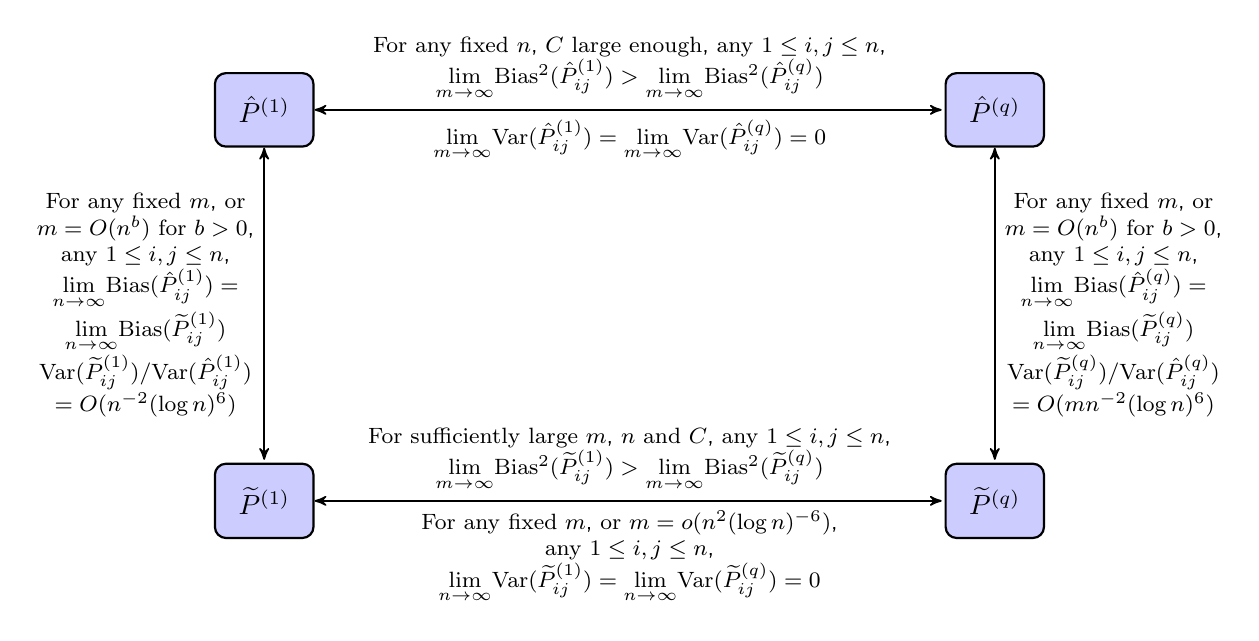
\begin{tikzpicture}[
  font=\sffamily,
  every matrix/.style={ampersand replacement=\&,column sep=2cm,row sep=2cm},
  block/.style={draw,thick,rounded corners,fill=blue!20,inner sep=.3cm},
  process/.style={draw,thick,circle,fill=blue!20},
  sink/.style={source,fill=green!20},
  datastore/.style={draw,very thick,shape=datastore,inner sep=.3cm},
  dots/.style={gray,scale=2},
  to/.style={->,>=stealth',shorten >=1pt,semithick,font=\sffamily\footnotesize},
  tofrom/.style={<->,>=stealth',shorten >=1pt,semithick,font=\sffamily\footnotesize},
  every node/.style={align=center}]

  % Position the nodes using a matrix layout
  \matrix{
    \node[block] (MLE) {$\hat{P}^{(1)}$};
      \& \& \& \& \node[block] (MLqE) {$\hat{P}^{(q)}$};\\
	\\
    \node[block] (XMLE) {$\widetilde{P}^{(1)}$};
      \& \& \& \& \node[block] (XMLqE) {$\widetilde{P}^{(q)}$}; \\
  };

  % Draw the arrows between the nodes and label them.
  \draw[tofrom] (MLE) -- node[midway,above] {$\mathrm{For}$ $\mathrm{any}$ $\mathrm{fixed}$ $n$, $C$ $\mathrm{large}$ $\mathrm{enough}$, $\mathrm{any}$ $1 \le i, j \le n$, \\$\underset{m \to \infty}{\lim} \mathrm{Bias}^2(\hat{P}_{ij}^{(1)}) > \underset{m \to \infty}{\lim} \mathrm{Bias}^2(\hat{P}_{ij}^{(q)})$}
      node[midway,below] {$\underset{m \to \infty}{\lim} \mathrm{Var}(\hat{P}_{ij}^{(1)}) = \underset{m \to \infty}{\lim} \mathrm{Var}(\hat{P}_{ij}^{(q)}) = 0$} (MLqE);
  \draw[tofrom] (MLE) -- node[midway,left] {$\mathrm{For}$ $\mathrm{any}$ $\mathrm{fixed}$ $m$, $\mathrm{or}$ \\ $m = O(n^b)$ $\mathrm{for}$ $b>0$, \\$\mathrm{any}$ $1 \le i, j \le n$, \\$\underset{n \to \infty}{\lim} \mathrm{Bias}(\hat{P}_{ij}^{(1)}) =$\\$ \underset{n \to \infty}{\lim} \mathrm{Bias}(\widetilde{P}_{ij}^{(1)})$\\$\mathrm{Var}(\widetilde{P}_{ij}^{(1)})/\mathrm{Var}(\hat{P}_{ij}^{(1)})$\\$ = O(n^{-2} (\log n)^6)$} (XMLE);
  \draw[tofrom] (MLqE) -- node[midway,right] {$\mathrm{For}$ $\mathrm{any}$ $\mathrm{fixed}$ $m$, $\mathrm{or}$ \\ $m = O(n^b)$ $\mathrm{for}$ $b>0$, \\$\mathrm{any}$ $1 \le i, j \le n$, \\$\underset{n \to \infty}{\lim} \mathrm{Bias}(\hat{P}_{ij}^{(q)}) = $\\$\underset{n \to \infty}{\lim} \mathrm{Bias}(\widetilde{P}_{ij}^{(q)})$\\$\mathrm{Var}(\widetilde{P}_{ij}^{(q)})/\mathrm{Var}(\hat{P}_{ij}^{(q)})$\\$= O(m n^{-2} (\log n)^6)$} (XMLqE);
  \draw[tofrom] (XMLE) -- node[midway,above] {$\mathrm{For}$ $\mathrm{sufficiently}$ $\mathrm{ large}$ $m$, $n$ $\mathrm{and}$ $C$, $\mathrm{any}$ $1 \le i, j \le n$, \\$\underset{m \to \infty}{\lim} \mathrm{Bias}^2(\widetilde{P}_{ij}^{(1)}) > \underset{m \to \infty}{\lim} \mathrm{Bias}^2(\widetilde{P}_{ij}^{(q)})$}
      node[midway,below] {$\mathrm{For}$ $\mathrm{any}$ $\mathrm{fixed}$ $m$, $\mathrm{or}$ $m = o(n^2 (\log n)^{-6})$, \\$\mathrm{any}$ $1 \le i, j \le n$, \\$\underset{n \to \infty}{\lim} \mathrm{Var}(\widetilde{P}_{ij}^{(1)}) = \underset{n \to \infty}{\lim} \mathrm{Var}(\widetilde{P}_{ij}^{(q)}) = 0$} (XMLqE);
\end{tikzpicture}
\end{center}
\caption{\label{fig:summary}Relationship between four estimators.}
\end{figure}






\section{Extensions}
\label{section:extension}
We can generalize both the exponential distribution and the entry-wise ML$q$E to an arbitrary $F$ and any entry-wise estimator $\hat{P}$ with the following assumptions:
\begin{itemize}
\item Let $A \stackrel{iid}{\sim} (1-\epsilon) F(P) + \epsilon F(C) $ and $H_{ij}^{(1)} = E[\hat{P}_{ij}^{(1)}] = (1-\epsilon) E_F(P_{ij}) + \epsilon E_F(C_{ij})$, then $E[(A_{ij} - H_{ij}^{(1)})^k] \le \mathrm{const} \cdot k!$.
\item There exists $C_0(P_{ij}, \epsilon) > 0$ such that under the contaminated model with $C > C_0(P_{ij}, \epsilon)$,
\[
	\lim_{m \to \infty} \left| E[\hat{P}_{ij}] - P_{ij} \right| < 
    \lim_{m \to \infty} \left| E[\hat{P}^{(1)}_{ij}] - P_{ij} \right|,
\]
for $1 \le i, j \le n$.
\item $\hat{P}_{ij} \le \mathrm{const} \cdot \hat{P}_{ij}^{(1)}$. This might be generalized to with high probability later.
\item $\mathrm{Var}(\hat{P}_{ij}) = O(m^{-1})$, where $m$ is the number of observations.
\end{itemize}

\section{Empirical Results}

\subsection{Simulation Results}

\begin{itemize}
\item We demonstrate the theoretical results in Section 3.1, the relative efficiency of $\hat{P}$, via various Monte Carlo simulation experiments.
\end{itemize}

\subsubsection{Simulation Setting}
\begin{itemize}
\item Here we consider the 2-block SBM parameterized by
\begin{equation*}
B = \begin{bmatrix}
4.2 & 2 \\
2 & 7
\end{bmatrix}
,\qquad \rho = \begin{bmatrix}
0.5 & 0.5
\end{bmatrix}.
\end{equation*}
\item The contamination is also a 2-block SBM parameterized by
\begin{equation*}
B = \begin{bmatrix}
20 & 18 \\
18 & 25
\end{bmatrix}
,\qquad \rho = \begin{bmatrix}
0.5 & 0.5
\end{bmatrix}.
\end{equation*}
\item And we embed the graphs into the dimension $d = \mathrm{rank}(B) = 2$.
\end{itemize}



\subsubsection{Simulation Results}
\begin{itemize}
\item Figure \ref{fig:eps} plots the mean squared error in average by varying contamination ratio $\epsilon$ with fixed $n = 100$ and $m = 10$ based on 1000 Monte Carlo replicates. And we use $q=0.8$ when applying ML$q$E.
Different colors represent the simulated MSE associated with four different estimators.
\textbf{1. MLE $\hat{P}^{(1)}$ vs ML$q$E $\hat{P}^{(q)}$:}
MLE outperforms a little bit when there is no contamination (i.e. $\epsilon = 0$), but it degrades dramatically when contamination increases;
\textbf{2. MLE $\hat{P}^{(1)}$ vs ASE o MLE $\widetilde{P}^{(1)}$: }
ASE procedure takes the low rank structure into account and $\widetilde{P}^{(1)}$ wins the bias-variance tradeoff;
\textbf{3. ML$q$E $\hat{P}^{(q)}$ vs ASE o ML$q$E $\widetilde{P}^{(q)}$: }
ML$q$E preserves the low rank structure of the original graph more or less, so ASE procedure still helps and $\widetilde{P}^{(q)}$ wins the bias-variance tradeoff;
\textbf{4. ASE o ML$q$E $\widetilde{P}^{(q)}$ vs ASE o MLE $\widetilde{P}^{(1)}$: }
When contamination is large enough, $\widetilde{P}^{(q)}$ based on ML$q$E is better, since it inherits the robustness from ML$q$E.
\item Figure \ref{fig:q} show the mean squared error in average by varying the parameter $q$ in ML$q$E with fixed $n = 100$, $m = 10$ and $\epsilon = 0.2$ based on 1000 Monte Carlo replicates. Different colors represent the simulated MSE associated with four different estimators.
1. ASE procedure takes advantage of the graph structure and improves the performance of the corresponding estimators;
2. ML$q$E shows the robustness property compare to the MLE. And as $q$ goes to 1, ML$q$E goes to the MLE as expected.
\item By comparing the performance of the four estimators based on different setting, we demonstrate the theoretical results in Section \ref{section:theory}.
\end{itemize}

\begin{figure}[!htb]
\centering
\includegraphics[width=1\textwidth]{eps.png}
\caption{Mean squared error in average by varying contamination ratio $\epsilon$ with fixed $n = 100$ and $m = 10$ based on 1000 Monte Carlo replicates. And we use $q=0.8$ when applying ML$q$E.
Different colors represent the simulated MSE associated with four different estimators.
\textbf{1. MLE $\hat{P}^{(1)}$ vs ML$q$E $\hat{P}^{(q)}$:}
MLE outperforms a little bit when there is no contamination (i.e. $\epsilon = 0$), but it degrades dramatically when contamination increases;
\textbf{2. MLE $\hat{P}^{(1)}$ vs ASE o MLE $\widetilde{P}^{(1)}$: }
ASE procedure takes the low rank structure into account and $\widetilde{P}^{(1)}$ wins the bias-variance tradeoff;
\textbf{3. ML$q$E $\hat{P}^{(q)}$ vs ASE o ML$q$E $\widetilde{P}^{(q)}$: }
ML$q$E preserves the low rank structure of the original graph more or less, so ASE procedure still helps and $\widetilde{P}^{(q)}$ wins the bias-variance tradeoff;
\textbf{4. ASE o ML$q$E $\widetilde{P}^{(q)}$ vs ASE o MLE $\widetilde{P}^{(1)}$: }
When contamination is large enough, $\widetilde{P}^{(q)}$ based on ML$q$E is better, since it inherits the robustness from ML$q$E.}
\label{fig:eps}
\end{figure}

\begin{figure}[!htb]
\centering
\includegraphics[width=1\textwidth]{q.png}
\caption{Mean squared error in average by varying the parameter $q$ in ML$q$E with fixed $n = 100$, $m = 10$ and $\epsilon = 0.2$ based on 1000 Monte Carlo replicates. Different colors represent the simulated MSE associated with four different estimators.
1. ASE procedure takes advantage of the graph structure and improves the performance of the corresponding estimators;
2. ML$q$E shows the robustness property compare to the MLE. And as $q$ goes to 1, ML$q$E goes to the MLE as expected.}
\label{fig:q}
\end{figure}

  
\begin{figure}
\centering
\includegraphics[width=0.8\textwidth]{Cluster.png}
\end{figure}



\subsection{CoRR Graphs}
\begin{itemize}
\item In practice, the graphs may not perfectly follow an RDPG, or even not IEM. But we are still interested in the discussed approach. To demonstrate that the estimates are still valid in such cases, we examine the datasets, CPAC200, which is a set of 454 brain connectomes with different number of nodes generated from fMRI scans available at the Consortium for Reliability and Reproducibility (CoRR).
\item The dataset has 454 different brain scans in the form of weighted, undirected graph with no self loop, based on the pipeline described in \cite{kiar2016graph} and \cite{neurodata}.
\item To compare the four estimators, we perform a cross-validation study on 454 graphs.
\item We run 1000 simulations on the dataset for each sample size $m = 1$, $m = 2$, $m = 5$. And we apply ASE for all possible dimensions, i.e. $d$ ranges from 1 to $n$. The result is shown in Figure \ref{fig:CPAC200}.
\item Since it is real data, ML$q$E outperforms ML$E$ because of the robustness property. Moreover, as suggested in the previous theorems, such property is kept after the ASE procedure.
\item When $d$ is small, ASE procedure underestimates the dimension and fail to get important information, which leads to poor performance. In practice, we use algorithms like Zhu and Ghodsi's method to select the dimension $d$. We can see Zhu and Ghodsi's algorithm does a pretty good job for selecting the dimension to embed.
\item When $m$ is small, MLE and ML$q$E have large variances which lead to large MSE. Meanwhile, the ASE procedure reduces the variance by taking advantages of the graph structure.
\end{itemize}

\begin{figure}
\centering
\includegraphics[width=0.8\textwidth]{CPAC200.png}
\caption{Comparison of mean squared error in average among four estimators while embedding the graphs into different dimensions with different size $m$ of the subsamples. The dimensions chosen by the 3d elbow of Zhu and Ghodsi are denoted in triangle and square. When $m$ is small, both robust estimation and ASE procedure help improving the performance, making $\widetilde{P}^{(q)}$ the best among four estimators.}
\label{fig:CPAC200}
\end{figure}





\section{Discussion}


\section{Appendix}

All proofs here.



\bibliography{Bib}{}
\bibliographystyle{plain}






%\newpage
%
%\section{Backup}
%
%
%\section{Discussion}
%
%\subsection{Summary}
%\begin{itemize}
%\item In this paper, we propose a better way to estimate the mean of a collection of graphs by taking advantage of the low rank structure of the graphs.
%\end{itemize}
%
%\subsection{Future Work}
%\begin{itemize}
%\item Generally the observations we have are always contaminated in practice. In this case, improved robust estimator based on the low rank structure of the graphs is preferred.
%\item Estimating the rank of the graph structure accurately will certainly help improve the results.
%\item In this paper, we are using Scheinerman's method with 1 iteration for diagonal augmentation.
%\end{itemize}
%
%
%
%
%
%
%\section{Methods}
%
%\subsection{Choosing Dimension}
%\label{section:dim_select}
%\begin{itemize}
%\item Often in dimensionality reduction techniques, the choice for dimension, d, relies on visually analyzing a plot of the ordered eigenvalues, looking for a ``gap'' or ``elbow'' in the scree-plot.
%\item USVT is a simple estimation procedure that works for any matrix that has ``a little bit of structure''.
%\end{itemize}
%
%\subsection{Graph Diagonal Augmentation}
%\begin{itemize}
%\item The graphs examined in this work are hollow, in that there are no self-loops and thus the diagonal entries of the adjacency matrix are 0. This leads to a bias in the calculation of the eigenvectors.
%\item We minimize this bias by using an iterative method developed by Scheinerman and Tucker.
%\end{itemize}
%
%\subsection{Source Code}
%
%\subsection{Dataset Description}
%\begin{itemize}
%\item The original dataset is from the Emotion and Creativity One Year Retest Dataset provided by Qiu, Zhang and Wei from Southwest University. It is comprised of 235 subjects, all of whom were college students. Each subject underwent two sessions of anatomical, resting state DTI scans, spaced one year apart. Due to the incomplete data, the true number of scans is 454.
%\item When deriving MR connectomes, the NeuroData team parcellate the brain into groups of nodes as defined by anatomical atlases. The atlases are defined either physiologically or structurally by neuroanatomists (Desikan and JHU), or are generated using a segmentation algorithm looking for certain features or groupings (CPAC200).
%\item The graphs we are using are processed by NeuroData team from DTI data of the original dataset generated with different atlases (desikan, JHU and CPAC200), each containing different region/node definitions.
%\item The graphs are undirected, unweighted and with no self-loops. An edge exists between two regions when there is at least one white-matter tract connecting the corresponding two parts of the brain.
%\end{itemize}
%
%\subsection{Outline for the Proof of the Theorems}



\end{document}